%!TeX program = xelatex
\documentclass[12pt,hyperref,a4paper,UTF8]{ctexart}
\usepackage{BNUpapers}
\usepackage{graphicx}
\usepackage{amsmath}
\usepackage{booktabs}
\usepackage{array}
\usepackage{float}
\usepackage{url}
\usepackage{tikz}
\usetikzlibrary{positioning,arrows.meta,shapes.geometric,calc}
\graphicspath{{assets/report_figures/}}

\renewcommand{\papertitlecn}{基于可复用 SVG 模板与多源数据仓库的自行车配件热力图可视化系统设计与实现}
\renewcommand{\papertitleen}{Design and Implementation of a Bicycle Component Heatmap Visualization System Based on Reusable SVG Templates and Multi-source Data Warehousing}
\renewcommand{\paperauthor}{课程项目作者}
\renewcommand{\paperinstitution}{北京师范大学}
\renewcommand{\papercourse}{《数据可视化》课程论文}
\renewcommand{\paperdate}{2026年6月}

%%-------------------------------正文开始---------------------------%%
\begin{document}

%%-----------------------封面--------------------%%
\cover

%%------------------摘要-------------%%
\begin{abstract}
针对自行车整车及配件数据来源分散、字段异构、部件语义不统一以及传统统计图难以表达结构差异的问题，本文设计并实现了一套基于可复用 SVG 模板与多源数据仓库的自行车配件热力图可视化系统。系统围绕“数据获取、统一建库、语义归一、模板设计、运行时渲染、工具化复用”六个环节展开：首先接入公开数据集、Bike Index API、品牌官网、配件目录、报价与评测来源，构建面向可视化任务的多源采集链路；其次采用 \texttt{raw--bronze--silver--gold} 分层数据仓库组织整车、部件、报价、评测、图像与标注等实体，并以标准部件 taxonomy 完成官网规格字段到模板槽位的映射；随后基于 Inkscape 手工设计公路车与山地车两套可复用 SVG 模板，建立 \texttt{partKey} 到 SVG 元素集合的一对多绑定关系；在此基础上，将原有单页展示重构为 \texttt{bike-template-engine} 统一运行时，并实现 \texttt{template studio} 与 \texttt{dataset mapper} 两个辅助工作台，使模板维护和新数据源接入从脚本级操作提升为协议级和配置级操作。实验结果表明，该系统能够稳定支持公路车与山地车模板切换、价格/质量/性价比多模式切换、部件点击联动、模板覆盖率提示以及品牌--部件矩阵展示，并在数据稀疏条件下通过显式标注的代表性回填策略维持可解释性。本文的主要贡献在于：提出了一种面向结构化对象的模板热力图可视化方法；构建了服务于该方法的统一数据协议与模板包规范；实现了从原型页面到可复用工具原型的系统化重构。该研究为后续接入图像识别、实例分割与插件化嵌入提供了稳定基础，也为《数据可视化》课程中的数据工程、视觉编码与交互设计提供了较完整的综合实践案例。
\end{abstract}

\noindent\textbf{关键词：} 自行车数据可视化；SVG 模板；数据仓库；热力图；模板引擎；交互设计

\vspace{1em}
\noindent\textbf{Abstract:} This paper presents a reusable bicycle component heatmap visualization system driven by multi-source data warehousing and SVG templates. The system integrates public datasets, open APIs, official brand specification pages, offer snapshots, and review signals into a unified layered warehouse, then maps heterogeneous fields into a standard part taxonomy and template protocol. Based on manually curated SVG templates for road and mountain bikes, the project builds a unified runtime named \texttt{bike-template-engine}, together with \texttt{template studio} and \texttt{dataset mapper}, to support template maintenance, protocol transformation, and reusable interactive delivery. Experimental results show that the system supports template switching, metric-mode switching, component-level interaction, explainable missing-data handling, and brand-part overview analysis. The work demonstrates a complete path from data acquisition to reusable domain visualization tooling.

\thispagestyle{empty}

%%--------------------------目录页------------------------%%
\newpage
\tableofcontents

%%------------------------正文页从这里开始-------------------%%
\newpage

\begin{center}
    {\Huge \textbf{基于可复用 SVG 模板与多源数据仓库的自行车配件热力图可视化系统设计与实现}}\\[0.8em]
    {\large Design and Implementation of a Bicycle Component Heatmap Visualization System Based on Reusable SVG Templates and Multi-source Data Warehousing}
\end{center}

\section{引言}

随着骑行文化、运动消费与微出行场景的持续发展，自行车产品已经从单一交通工具演化为具有显著结构差异和配件生态的复杂消费品。对于普通用户、课程评审者乃至研究者而言，真正需要理解的往往不是一辆车的总价，而是“哪些部件决定了这辆车的价值结构”“不同品牌在相同部件位置上的配置差异是什么”“宣传文案中的复杂规格信息如何被转换为可解释的结构认知”。然而，现实中的自行车数据大多以官网规格表、开放 API 文本记录、配件目录、评测页面或图像数据集的形式分散存在，字段粒度、命名方式与结构组织差异极大，导致直接使用传统柱状图、饼图或表格难以充分表达结构对象本身。

从数据可视化研究的视角看，合适的可视表达应当与对象结构、任务目标和用户认知方式保持一致 \cite{Munzner2014,Tufte2001,Ware2020}。自行车是一类天然具有空间结构和部件语义的对象，价格、质量与性价比等指标并不是孤立存在的数值，而是附着于车架、前叉、轮胎、传动、制动和坐垫等具体部件之上。如果仍以传统统计视图为唯一表达手段，用户必须在脑中重复完成“字段名称 $\rightarrow$ 部件位置 $\rightarrow$ 价值理解”的转换过程，认知负担较重，不利于课堂展示和研究阐释。

因此，本文将问题进一步抽象为：能否建立一种围绕标准结构模板的、可复用的、面向领域对象的可视化系统，使多源异构自行车数据能够被映射到统一的空间语义骨架之上，并支持多维指标切换、部件级交互以及后续工具化复用？围绕这一问题，本文并未停留在单一前端页面的制作，而是从数据获取、数据治理、数据库设计、模板建模、协议抽象、运行时重构和页面交付等多个层面系统推进。

本文的主要工作与贡献可概括为以下三个方面。第一，面向自行车整车与配件场景，构建了覆盖公开数据集、开放 API、品牌官网、报价和评测来源的多源采集与分层仓库体系，并围绕标准部件 taxonomy 建立统一实体设计。第二，基于 Inkscape 手工设计并维护两套可复用 SVG 模板，提出面向模板热力图的标准协议与模板包规范，使部件映射、颜色编码和缺失状态表达具备长期可维护性。第三，将原始展示页系统重构为 \texttt{bike-template-engine} 统一运行时，并实现 \texttt{template studio} 与 \texttt{dataset mapper}，使系统从一次性展示原型升级为可扩展、可维护的领域可视化工具原型。

全文结构安排如下。第二节回顾相关研究与工具背景；第三节阐述系统目标与总体架构；第四节介绍多源数据获取和仓库建设过程；第五节讨论标准协议、模板设计与视觉编码；第六节说明统一运行时与前后端实现；第七节给出实验结果与页面展示；第八节总结局限性与未来工作；第九节给出全文结论。

\section{相关工作}

\subsection{数据可视化理论与领域对象表达}

数据可视化研究长期强调视觉编码与任务匹配的重要性。Tufte 指出高质量信息图应减少不必要装饰并强化数据与结构表达 \cite{Tufte2001}；Munzner 从任务、数据类型和编码机制出发，系统提出了可视化设计的多层抽象框架 \cite{Munzner2014}；Ware 则从认知心理学角度说明空间位置、颜色和形状是影响理解效率的重要视觉变量 \cite{Ware2020}。这些研究提示我们，若对象本身具有明显的结构轮廓，则可视化不必局限于笛卡尔坐标系，也可以将对象模板作为信息承载空间。

对于需要同时表达结构位置和数值差异的场景，结构模板驱动的可视化方案具有明显优势。例如医学解剖图、工业设备监控图和流程图式仪表板，都在实践中证明了“对象空间本身就是视觉空间”的可行性。自行车与这些对象类似，天然具有可分解的部件结构，因此特别适合采用模板热力图方式进行表达。

\subsection{BI 工具与可复用图形组件启发}

近年来，FineReport、FineBI、Power BI 等 BI 工具逐步从固定图表走向可复用、可嵌入、可交互的图形组件体系。这些系统普遍强调数据源标准化、图形容器复用、图例切换、条件着色和多视图联动等能力。尽管它们很少直接针对自行车结构对象设计模板，但其“图形作为组件、数据通过协议驱动、交互由状态管理统一组织”的思想，对本研究具有直接启发作用。本文最终形成的 \texttt{bike-template-engine}、\texttt{template studio} 与 \texttt{dataset mapper} 三层形态，本质上正是将 BI 组件化思路迁移到领域模板可视化场景中。

\subsection{公开数据集与视觉扩展背景}

在后续计算机视觉扩展方面，DelftBikes、BBBicycles、GeoBIKED 等公开数据集提供了自行车图像、部件结构或损伤识别等相关资源。虽然本文工作的主线并非直接训练识别模型，但这些数据集为未来实现“用户上传图片 $\rightarrow$ 部件识别 $\rightarrow$ 模板对齐 $\rightarrow$ 热力图生成”的闭环提供了可行的数据入口。因此，本系统并不是与视觉理解路线相分离的展示工程，而是为后续视觉扩展预留了标准化接口与资产组织方式。

\section{系统目标与总体架构}

\subsection{系统目标}

本文系统的总体目标，是构建一套基于可复用 SVG 模板的自行车配件热力图可视化系统，使来自多源异构环境的整车与部件数据能够经过统一治理后，以价格、质量和性价比等多维视角映射到稳定的结构语义空间中，并通过统一运行时向网页、报告和后续嵌入场景进行交付。该目标进一步细化为以下几个方面：

\begin{enumerate}
    \item 建立覆盖多来源的可扩展数据获取链路，而非依赖单一站点或单一接口；
    \item 构建服务于可视化任务的数据仓库分层和统一实体设计；
    \item 设计标准部件 taxonomy 与模板协议，稳定描述部件语义与可视区域关系；
    \item 设计公路车与山地车两套可复用 SVG 模板，并保证可维护性；
    \item 实现统一运行时，支持多指标模式切换、部件点击联动和缺失提示；
    \item 将系统进一步工具化，支持模板维护与新数据源快速接入。
\end{enumerate}

\subsection{总体架构}

为了形成从数据源到页面交付的完整闭环，本文采用“数据层、协议层、模板层、运行时层、交付层”五层结构。图 \ref{fig:architecture} 给出了系统总体架构。

\begin{figure}[H]
    \centering
    \resizebox{0.98\textwidth}{!}{%
    \begin{tikzpicture}[
        font=\small,
        node distance=10mm and 8mm,
        box/.style={draw, rounded corners, align=center, minimum width=30mm, minimum height=10mm},
        line/.style={-Latex, thick}
    ]
        \node[box] (source) {外部数据源\\官网 / API / 数据集 / 评测};
        \node[box, right=of source] (mapper) {dataset mapper\\字段映射 / 清洗 / 归一};
        \node[box, right=of mapper] (protocol) {标准协议层\\bike payload / metrics / evidence};
        \node[box, below=of mapper] (studio) {template studio\\标签维护 / 映射维护 / 预览};
        \node[box, below=of protocol] (package) {template package\\template.svg / mapping / theme};
        \node[box, right=18mm of protocol] (engine) {bike-template-engine\\renderer / state / interaction};
        \node[box, above right=8mm and 12mm of engine] (web) {Web 页面\\主页面 / 报告 / 工作台};
        \node[box, below right=8mm and 12mm of engine] (embed) {Embed 输出\\iframe / SDK / 插件};

        \draw[line] (source) -- (mapper);
        \draw[line] (mapper) -- (protocol);
        \draw[line] (studio) -- (package);
        \draw[line] (protocol) -- (engine);
        \draw[line] (package) -- (engine);
        \draw[line] (engine) -- (web);
        \draw[line] (engine) -- (embed);
        \draw[line] (mapper) -- (studio);
    \end{tikzpicture}
    }
    \caption{系统总体架构}
    \label{fig:architecture}
\end{figure}

该架构的关键在于实现数据与模板的解耦。外部数据源不直接驱动页面，而是先通过 \texttt{dataset mapper} 转化为标准协议；模板资产也不被硬编码在单页脚本中，而是被封装为模板包。统一运行时只消费标准协议和模板包，从而使新模板、新数据源和新交付方式都能够在不重写核心渲染逻辑的前提下持续扩展。

\section{多源数据获取与数据仓库建设}

\subsection{数据来源设计}

为了保证系统既有足够的样本覆盖，又具备部件级信息的解释力，本文采用多源数据获取方案。各类数据源承担的角色如表 \ref{tab:sources} 所示。

\begin{table}[H]
    \centering
    \small
    \begin{tabular}{p{3.2cm} p{4.2cm} p{5.5cm}}
        \toprule
        数据来源类型 & 代表来源 & 主要作用 \\
        \midrule
        公开图像与标注数据集 & DelftBikes, BBBicycles, GeoBIKED & 为后续视觉识别、部件定位与标注资产管理提供基础资源 \\
        开放整车接口 & Bike Index API & 扩大整车样本覆盖面，补充车型、品牌与文本记录 \\
        品牌官网 & Giant, Merida, Trek, Canyon, Cannondale, Specialized 等 & 提供最接近真实产品配置的官方规格与结构字段 \\
        配件目录与报价来源 & 公开配件目录、价格页面 & 提供价格区间、平台信息和零部件商品证据 \\
        评测来源 & 公开评测站点、评分页面 & 提供质量评价、评论数量和外部口碑信号 \\
        \bottomrule
    \end{tabular}
    \caption{系统采用的主要数据来源及其作用}
    \label{tab:sources}
\end{table}

选择多源方案的根本原因在于，单一来源很难同时满足“车型覆盖广、部件信息细、价格证据足、质量信号可比较、图像资产可复用”等多个目标。官方规格最接近真实配置，但未必包含价格与评分；公开 API 样本量大，但字段粒度不稳定；评测与报价来源信号丰富，却往往缺少完整整车上下文。因此，只有通过仓库化组织多源数据，才能在后续导出中形成相对完整、可解释的结构化结果。

\subsection{采集流程与增量扩抓策略}

为了减少一次性全量抓取带来的维护成本，本文在采集层采用增量扩抓策略。对于开放 API，围绕公路、山地、折叠、通勤、电助力等关键词进行多轮扩抓，逐步扩大整车样本范围；对于品牌官网，则使用站点级过滤、目录级下钻与页面结构判别相结合的方式，尽可能提取真实产品页而非营销页或系列聚合页；对于组件品牌与评测来源，则以标准部件槽位为线索收集价格与评价信号，供后续指标计算使用。

图 \ref{fig:data-pipeline} 展示了数据获取与分层处理主流程。

\begin{figure}[H]
    \centering
    \begin{tikzpicture}[
        font=\small,
        node distance=8mm and 8mm,
        box/.style={draw, rounded corners, align=center, minimum width=28mm, minimum height=9mm},
        line/.style={-Latex, thick}
    ]
        \node[box] (a) {公开数据集};
        \node[box, right=of a] (b) {开放 API};
        \node[box, right=of b] (c) {品牌官网};
        \node[box, right=of c] (d) {报价 / 评测};

        \node[box, below=of b, minimum width=38mm] (raw) {Raw\\原始页面 / 接口 / 文件};
        \node[box, below=of raw, minimum width=38mm] (bronze) {Bronze\\轻清洗 / 去重 / 来源保留};
        \node[box, below=of bronze, minimum width=38mm] (silver) {Silver\\实体抽取 / 字段归一 / taxonomy 映射};
        \node[box, below=of silver, minimum width=38mm] (gold) {Gold\\统一导出 / API / engine payload};

        \draw[line] (a.south) |- (raw.north);
        \draw[line] (b.south) -- (raw.north);
        \draw[line] (c.south) |- (raw.north);
        \draw[line] (d.south) |- (raw.north);
        \draw[line] (raw) -- (bronze);
        \draw[line] (bronze) -- (silver);
        \draw[line] (silver) -- (gold);
    \end{tikzpicture}
    \caption{数据获取与分层处理流程}
    \label{fig:data-pipeline}
\end{figure}

\subsection{数据仓库分层设计}

本文采用 \texttt{raw--bronze--silver--gold} 四层设计组织数据资产。Raw 层保存原始网页、接口返回、下载文件和外部注释资源，以便问题回溯；Bronze 层完成轻量结构抽取、编码统一和基础去重；Silver 层着重建立实体关系、完成字段归一和标准部件槽位映射；Gold 层则直接面向可视化页面、工作台和引擎运行时进行导出。这种分层方式的优势主要体现在三点：其一，前端问题能够追溯到上游清洗规则；其二，数据规则更新时可以从中间层重建，而非重复抓取所有原始页面；其三，不同下游任务能够共享同一套中间资产。

\subsection{统一实体设计}

在数据库实体层，本文围绕整车、部件、外部证据与图像资产建立统一关系。核心实体包括：表示具体车型的 \texttt{bike\_variant}，沉淀标准部件目录的 \texttt{component\_catalog}，记录价格和来源快照的 \texttt{offer\_snapshot}，记录评分与评论目标的 \texttt{review\_target}，以及表示图像、标注集合和标注对象的 \texttt{image\_item}、\texttt{annotation\_set} 和 \texttt{annotated\_object}。与此同时，\texttt{part\_taxonomy} 作为语义主键，贯穿官网抽取、模板设计和运行时渲染的全过程。

这一设计避免了将整车规格、配件商品、评测文本和图像资源简单塞入单一大表的做法，使系统在处理“同一部件既是整车配置、又可能是独立商品、还可能是图像标注对象”的复杂情况时仍然保持语义清晰。

\section{标准协议、模板建模与视觉编码}

\subsection{标准部件 taxonomy 与协议设计}

将多源数据映射到模板热力图的前提，是为系统定义稳定的部件语义集合。本文围绕自行车结构特点定义了一套标准部件键，包括 \texttt{frame}、\texttt{fork}、\texttt{shock}、\texttt{brake}、\texttt{tyre}、\texttt{wheel}、\texttt{saddle}、\texttt{seatpost}、\texttt{handlebar}、\texttt{crankset}、\texttt{derailleur}、\texttt{cassette}、\texttt{chain}、\texttt{shifter}、\texttt{pedal} 等。上游官网字段无论写作 \texttt{Groupset}、\texttt{Frame Technology}、\texttt{Dropper Post} 还是 \texttt{Wheelset}，都需先被归一到标准部件槽位后，才能进入模板与页面。

围绕这一语义集合，系统定义了面向运行时的标准载荷。每一辆车的标准 payload 至少包含：整车基本信息、品牌与车型类型、模板类型、部件集合、各部件的证据强度以及价格、质量、性价比等指标。在部件层，除了 \texttt{partKey}、\texttt{displayName} 和 \texttt{componentName} 外，还维护 \texttt{templateLabels}、\texttt{sourceType}、\texttt{evidence} 与 \texttt{render} 等字段，使数据层、模板层与前端层之间形成稳定边界。

\subsection{Inkscape 模板设计与模板包规范}

为了保证结构语义的稳定性，本文没有直接依赖真实照片作为主可视载体，而是通过 Inkscape 手工设计并标注公路车与山地车两套可复用 SVG 模板。模板设计过程包括：提取标准侧视轮廓、拆分车架、前叉、轮胎、刹车、传动、把组、坐垫、座管和避震等局部结构、为路径与图层设置稳定标签，并在运行时反复验证着色和交互效果后进行修订。

进一步地，本文没有把模板仅仅作为一张 SVG 图片保存，而是将其组织为模板包。一个模板包至少包含 \texttt{template.svg}、\texttt{mapping.json}、\texttt{theme.json}、\texttt{schema.json}、\texttt{preview.svg} 与包级元信息。这样做的意义在于，使模板从“前端内部资源”升级为“可版本化、可验证、可维护的正式资产”。

\subsection{一对多映射与缺失表达}

实际部件与 SVG 路径之间并非一一对应关系。例如，车架通常由多个路径片段共同构成；刹车既可能涉及卡钳，也可能涉及刹把；山地车的避震则同时关联前叉和后避震两个位置。因此，本文采用 \texttt{partKey} 对应 \texttt{svg id[]} 的一对多映射设计。该设计既提升了视觉完整性，也使模板维护具备足够灵活性。

另一方面，模板热力图必须诚实面对数据缺失。若某一车型在特定部件上没有可靠数据，系统不会直接伪造真实部件，而是采用两级策略：优先保留“模板区域存在但当前无数据”的状态表达；仅在极度稀疏且影响整体可读性时，才使用明确标记的代表性回填项进行占位。这样既保证了可视化结果的可读性，也避免误导用户把推断值当作官方配置。

\subsection{指标计算与颜色编码}

本文的核心可视指标包括价格、质量和性价比三个维度。价格主要来自报价快照及其聚合结果，质量主要由评测、评论数量和来源可信度综合表征，性价比则体现价格与质量之间的平衡。为了在不同车型和部件之间获得可比较的颜色编码，系统对指标进行归一化处理。设部件 $p$ 在模式 $m$ 下的原始指标值为 $x_{m,p}$，则其归一化结果写为
\begin{equation}
\hat{x}_{m,p} = \frac{x_{m,p} - \min(x_m)}{\max(x_m) - \min(x_m) + \varepsilon},
\label{eq:norm}
\end{equation}
其中 $\varepsilon$ 为避免分母为零的稳定项。根据不同模式，系统分别采用暖色、冷色和青绿色系进行颜色映射，并将缺失状态保持为低饱和浅灰色，以强化数据完备度和数值强弱之间的区分。

\section{统一运行时与系统实现}

\subsection{从单页展示到统一运行时}

项目初期的页面生成逻辑主要集中在原始展示页脚本中，模板读取、数据拼接、颜色计算、图例切换和详情卡联动高度耦合。随着公路车与山地车模板共存、品牌矩阵与辅助工作台逐步加入，这种单页实现很快暴露出维护成本高、扩展困难和兼容性差的问题。因此，本文将展示系统进一步抽象为 \texttt{bike-template-engine} 统一运行时。该运行时只消费两类输入：标准协议载荷与模板包。所有页面交互、颜色构建和渲染状态生成都在统一接口下完成。

\subsection{运行时流程}

统一运行时的主要工作包括：根据车型选择模板类型，根据模式计算颜色映射，根据证据强度和缺失情况生成渲染状态，根据部件列表构造详情卡与说明项，并组织品牌--部件矩阵等辅助视图。图 \ref{fig:runtime} 给出了运行时主流程。

\begin{figure}[H]
    \centering
    \begin{tikzpicture}[
        font=\small,
        node distance=9mm and 8mm,
        box/.style={draw, rounded corners, align=center, minimum width=32mm, minimum height=9mm},
        line/.style={-Latex, thick}
    ]
        \node[box] (payload) {标准 bike payload};
        \node[box, right=of payload] (template) {模板包\\SVG / mapping / theme};
        \node[box, right=of template] (mode) {模式选择\\价格 / 质量 / 性价比};
        \node[box, below=of template] (state) {渲染状态构建\\颜色 / 覆盖率 / 缺失标记};
        \node[box, below left=of state] (detail) {详情卡摘要};
        \node[box, below=of state] (matrix) {品牌--部件矩阵};
        \node[box, below right=of state] (stage) {SVG 舞台渲染\\hover / click / 动画};

        \draw[line] (payload) -- (state);
        \draw[line] (template) -- (state);
        \draw[line] (mode) -- (state);
        \draw[line] (state) -- (detail);
        \draw[line] (state) -- (matrix);
        \draw[line] (state) -- (stage);
    \end{tikzpicture}
    \caption{统一运行时主流程}
    \label{fig:runtime}
\end{figure}

\subsection{Template Studio 与 Dataset Mapper}

为了让系统具备真正的复用能力，本文没有将模板维护与数据适配仍然保留为脚本层操作，而是实现了两个辅助工作台。\texttt{template studio} 负责可视化查看 SVG 元素、维护部件与元素映射、检查未绑定区域以及预览着色效果；\texttt{dataset mapper} 则负责将新来源 JSON 映射到标准协议，辅助开发者校验标准部件键、模板标签和指标字段的完整性。它们的存在使系统从“作者自己能够维护的页面”升级为“他人也能接着扩展的工具”。

\subsection{前端交互实现}

在页面交互层，系统支持车型选择、指标模式切换、部件点击联动、列表与模板双向高亮、缺失说明提示以及带有浮动放大效果的 SVG 动画。为保证交互与渲染逻辑的一致性，系统在运行时为模板区域显式注入查询属性，并通过统一状态管理控制选中态、悬停态和弱化态，从而解决了 SVG 场景中事件绑定不稳定的问题。对存在模板但暂无真实数据的区域，系统不再保持完全静默，而是提供“模板存在但当前车型缺失数据”的说明卡，使用户能够区分“交互无效”与“数据缺失”这两种完全不同的情况。

\section{实验结果与页面展示}

\subsection{实验设置与评价维度}

本文的实验更强调系统工程完整性与可解释性，而非单一数值指标的极致优化。因此，评价维度主要包括以下几个方面：其一，多源数据是否能够被稳定映射到统一仓库与标准协议；其二，模板热力图是否能够在公路车与山地车两类结构上保持稳定切换；其三，价格、质量和性价比三种模式是否能够在同一空间结构上形成一致而可解释的颜色表达；其四，页面交互是否能够帮助用户从总览快速进入部件层细节；其五，在数据稀疏情形下，系统是否能够保持诚实表达并尽量避免误导。

\subsection{主页面结果}

图 \ref{fig:engine-page} 展示了统一运行时主页面。可以看到，系统已经形成“模板舞台 + 模式控制 + 详情卡 + 部件列表 + 辅助矩阵”的综合页面结构。相较于单纯的着色 SVG，该页面更强调从总览到细节的阅读路径：用户先通过颜色快速感知整车结构的价值差异，再通过点击部件和详情卡进一步理解具体配置与证据强度。

\begin{figure}[H]
    \centering
    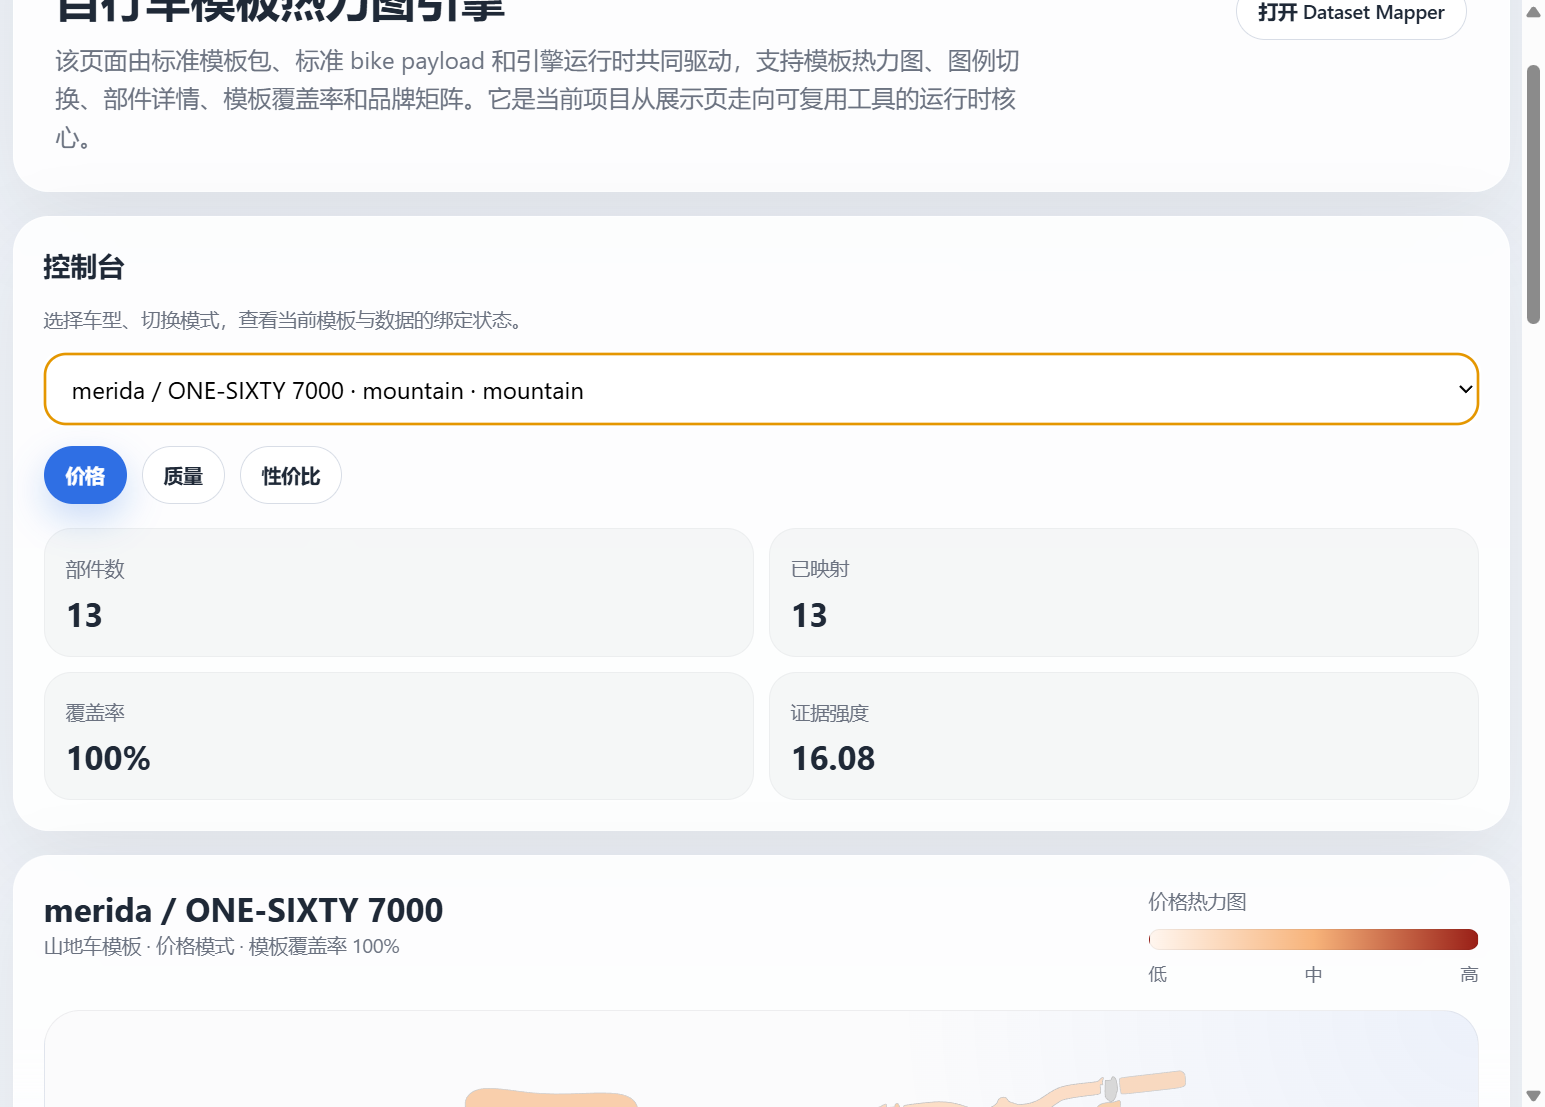
\includegraphics[width=0.90\textwidth]{engine_runtime_page.png}
    \caption{\texttt{bike-template-engine} 主页面}
    \label{fig:engine-page}
\end{figure}

\subsection{模板维护与数据映射工作台结果}

图 \ref{fig:studio-page} 和图 \ref{fig:mapper-page} 分别给出了模板工作台与数据映射工作台页面。前者使模板即资产、映射即配置的思想可视化；后者则展示了新数据源如何被规范化为统一协议。这两个页面的重要性在于，它们不仅展示最终结果，还展示结果的生产过程与维护机制。

\begin{figure}[H]
    \centering
    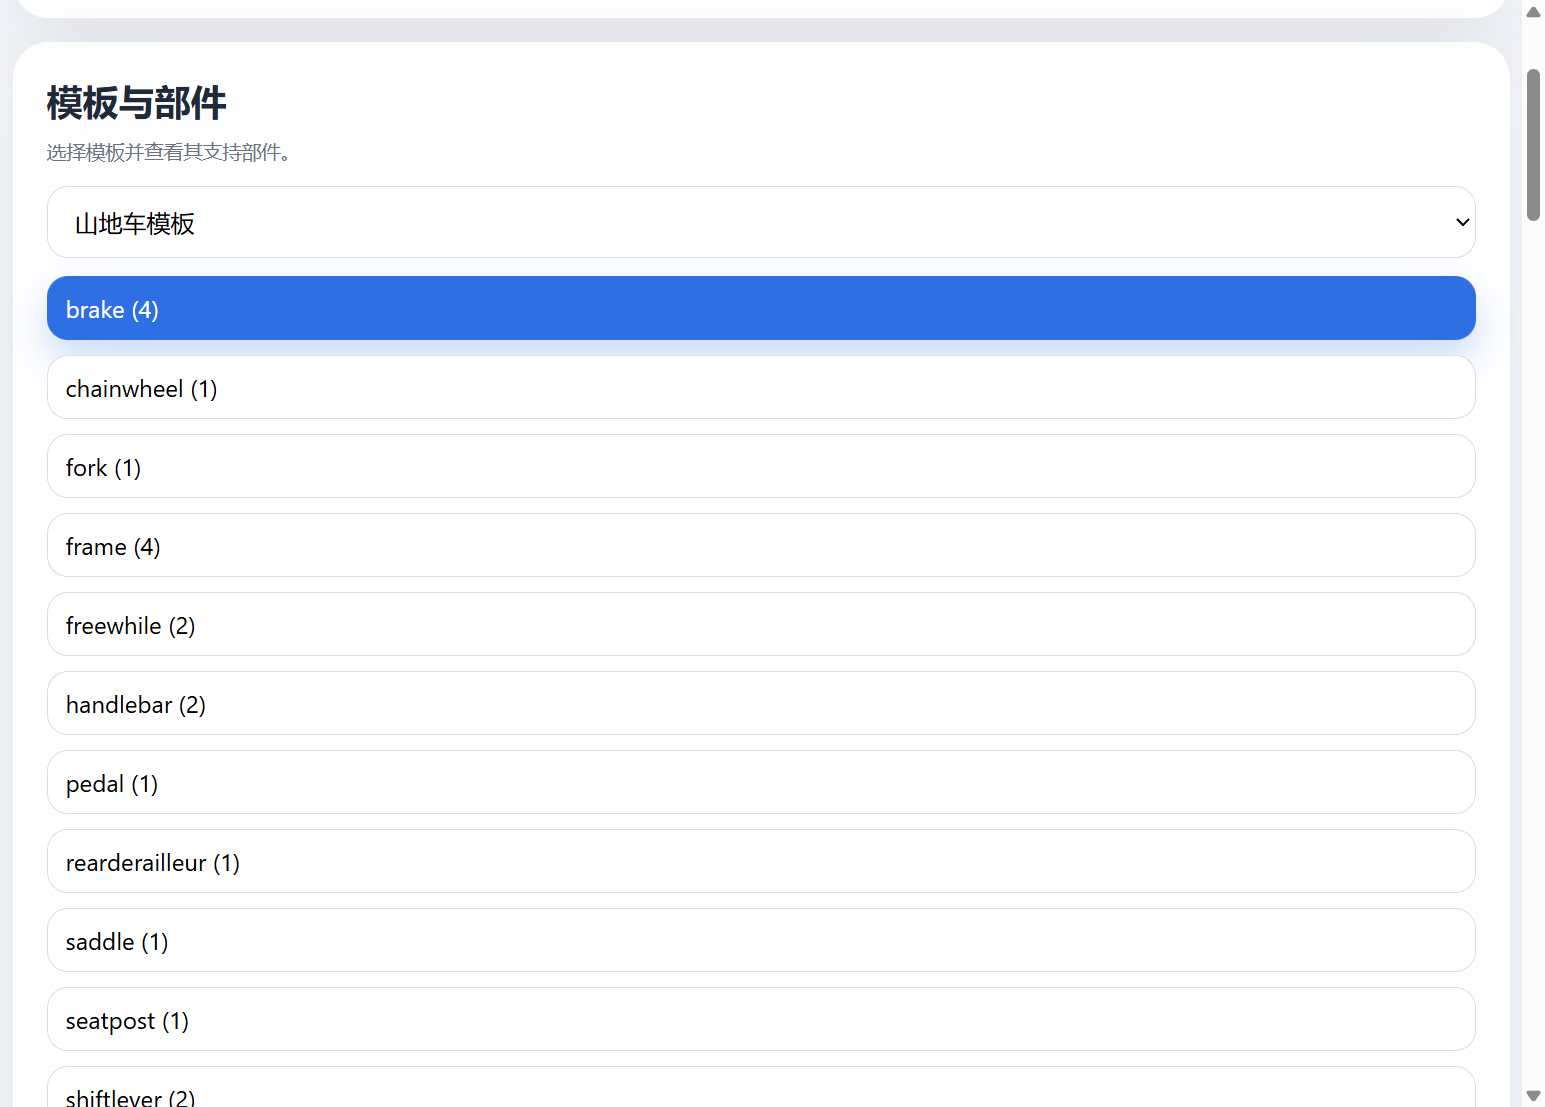
\includegraphics[width=0.88\textwidth]{template_studio_page.png}
    \caption{\texttt{template studio} 页面}
    \label{fig:studio-page}
\end{figure}

\begin{figure}[H]
    \centering
    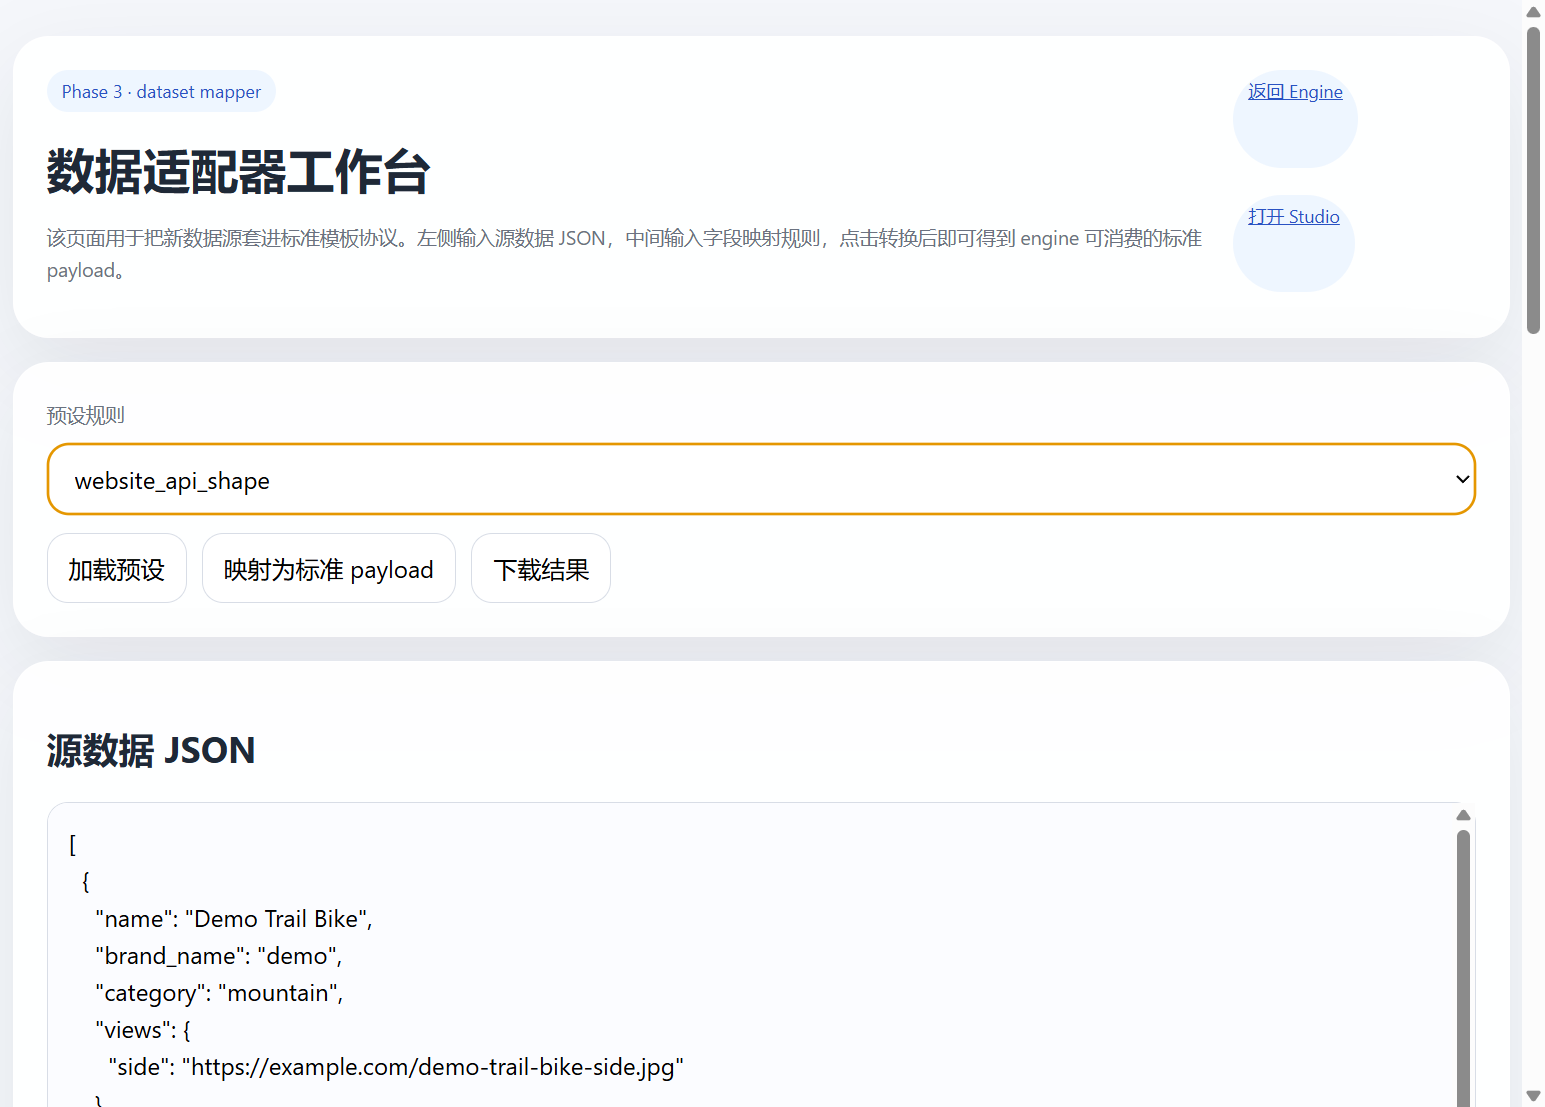
\includegraphics[width=0.88\textwidth]{dataset_mapper_page.png}
    \caption{\texttt{dataset mapper} 页面}
    \label{fig:mapper-page}
\end{figure}

\subsection{结果分析}

实验结果表明，本文系统在以下几个方面取得了较为稳定的效果。首先，在数据层，系统已经能够持续接入多源异构数据，并通过统一仓库导出页面 API 与引擎 payload，这意味着前端不再依赖人工拼装的样例数据。其次，在模板层，公路车与山地车模板已经形成相对稳定的双模板机制，使同一协议能够在不同结构骨架上复用。再次，在交互层，部件点击、模式切换、模板高亮与详情卡切换已经能够稳定协同工作，且对缺失数据区域提供了明确解释。最后，在工具化层，\texttt{bike-template-engine}、\texttt{template studio} 和 \texttt{dataset mapper} 的组合使系统从课程展示页面升级为具有后续维护与扩展能力的工具原型。

需要指出的是，系统在 Merida 等品牌上仍会受到官方规格稀疏的影响，部分车型只能依赖代表性回填项维持基本可读性。与其伪造完整配置，本文更强调显式标注缺失与回填来源，从而保持可视化结果的诚实性和解释性。

\section{讨论与局限性}

\subsection{数据治理比页面样式更关键}

本研究的一个重要经验是，许多表面上看似前端渲染失败的问题，本质上都源自数据治理不足。例如山地车大面积灰化问题，最终并非由颜色函数错误导致，而是由部件记录稀缺、模板标签不全、营销性规格字段污染以及组件页误入整车集合等多种数据层问题共同造成。这说明在领域可视化系统中，数据治理往往比单纯的页面美化更决定系统成败。

\subsection{模板驱动方案的边界}

模板热力图方案的优势在于稳定、可解释、便于报告和答辩展示，但其边界同样明显。首先，它依赖高质量模板设计，新车型或特殊结构加入时需要额外模板维护成本；其次，它难以直接覆盖任意拍摄角度和任意姿态的真实照片；再次，当数据严重缺失时，即使有代表性回填策略，也必须谨慎处理以避免误导。因此，模板驱动方案更适合作为“稳定表达骨架”，而不是对所有视觉场景的一次性终极解决方案。

\subsection{未来工作}

未来工作可从三个方向继续推进。第一，继续增强品牌官网采集与实体抽取规则，尤其针对 Trek、Cannondale、Canyon、Merida 等品牌补充更丰富的真实部件证据。第二，继续提升模板工具化程度，例如引入模板版本管理、自动发现未绑定元素、映射规则校验和更多车型模板。第三，结合公开数据集和已有标注流程，探索用户上传实拍侧视图后自动识别部件、完成模板配准并生成个性化热力图的全闭环系统。届时，本文构建的标准协议和模板包规范将成为连接视觉识别与可视交付的重要中间层。

\section{结论}

本文围绕自行车整车与配件数据的结构化可视表达问题，设计并实现了一套基于可复用 SVG 模板与多源数据仓库的热力图可视化系统。通过建立多源采集链路、分层数据仓库、标准部件 taxonomy、模板包规范与统一运行时，系统能够在公路车和山地车两类模板上稳定表达价格、质量和性价比等多维指标，并通过部件级交互提升可解释性。同时，本文将原始展示页系统进一步重构为 \texttt{bike-template-engine}、\texttt{template studio} 和 \texttt{dataset mapper} 三层工具体系，使系统具备了持续维护和扩展的基础。

对于《数据可视化》课程而言，本文工作的价值不仅在于展示了一个较完整的网页原型，更在于完整呈现了从数据源接入、字段归一、数据库设计、模板建模、视觉编码到交互实现和文档化表达的全过程。实践表明，结构化对象可视化并不只是“换一种画法”，而是需要数据工程、图形设计和系统抽象共同支撑的系统工程。该研究为后续进一步走向图像识别驱动的个性化可视化和插件化领域图形组件提供了稳定基础。

%%----------- 参考文献 -------------------%%
\begin{thebibliography}{99}
\bibitem{Tufte2001}
Edward R. Tufte. \textit{The Visual Display of Quantitative Information}. Graphics Press, 2nd edition, 2001.

\bibitem{Munzner2014}
Tamara Munzner. \textit{Visualization Analysis and Design}. CRC Press, 2014.

\bibitem{Ware2020}
Colin Ware. \textit{Information Visualization: Perception for Design}. Morgan Kaufmann, 4th edition, 2020.

\bibitem{Mackinlay1986}
Jock D. Mackinlay. Automating the design of graphical presentations of relational information. \textit{ACM Transactions on Graphics}, 5(2):110--141, 1986.

\bibitem{Heer2012}
Jeffrey Heer and Ben Shneiderman. Interactive dynamics for visual analysis. \textit{Communications of the ACM}, 55(4):45--54, 2012.

\bibitem{Segel2010}
Edward Segel and Jeffrey Heer. Narrative visualization: Telling stories with data. \textit{IEEE Transactions on Visualization and Computer Graphics}, 16(6):1139--1148, 2010.

\bibitem{BikeIndex}
Bike Index API. \url{https://bikeindex.org/documentation/api_v3}. Accessed 2026-06-10.

\bibitem{DelftBikes}
DelftBikes Dataset. TU Delft bicycle component dataset resource. Accessed 2026-06-10.

\bibitem{BBBicycles}
Bent \& Broken Bicycles Dataset. Public bicycle damage recognition dataset resource. Accessed 2026-06-10.

\bibitem{GeoBIKED}
GeoBIKED Dataset. Public bicycle image and annotation resource. Accessed 2026-06-10.

\bibitem{PowerBI}
Microsoft Power BI documentation. Custom visuals and report design resources. \url{https://learn.microsoft.com/power-bi/}. Accessed 2026-06-10.

\bibitem{FineBI}
FineBI / FineReport official documentation. Reusable visualization component design resources. Accessed 2026-06-10.
\end{thebibliography}

\end{document}
